\documentclass[border=10pt]{standalone}

\usepackage{tikz}
\usepackage{tikzsymbols}
\usetikzlibrary{calc,patterns,shapes.geometric}

\def\centerarc[#1](#2)(#3:#4:#5){\draw[#1] ($(#2)+({#5*cos(#3)},{#5*sin(#3)})$) arc (#3:#4:#5);}

\begin{document}
	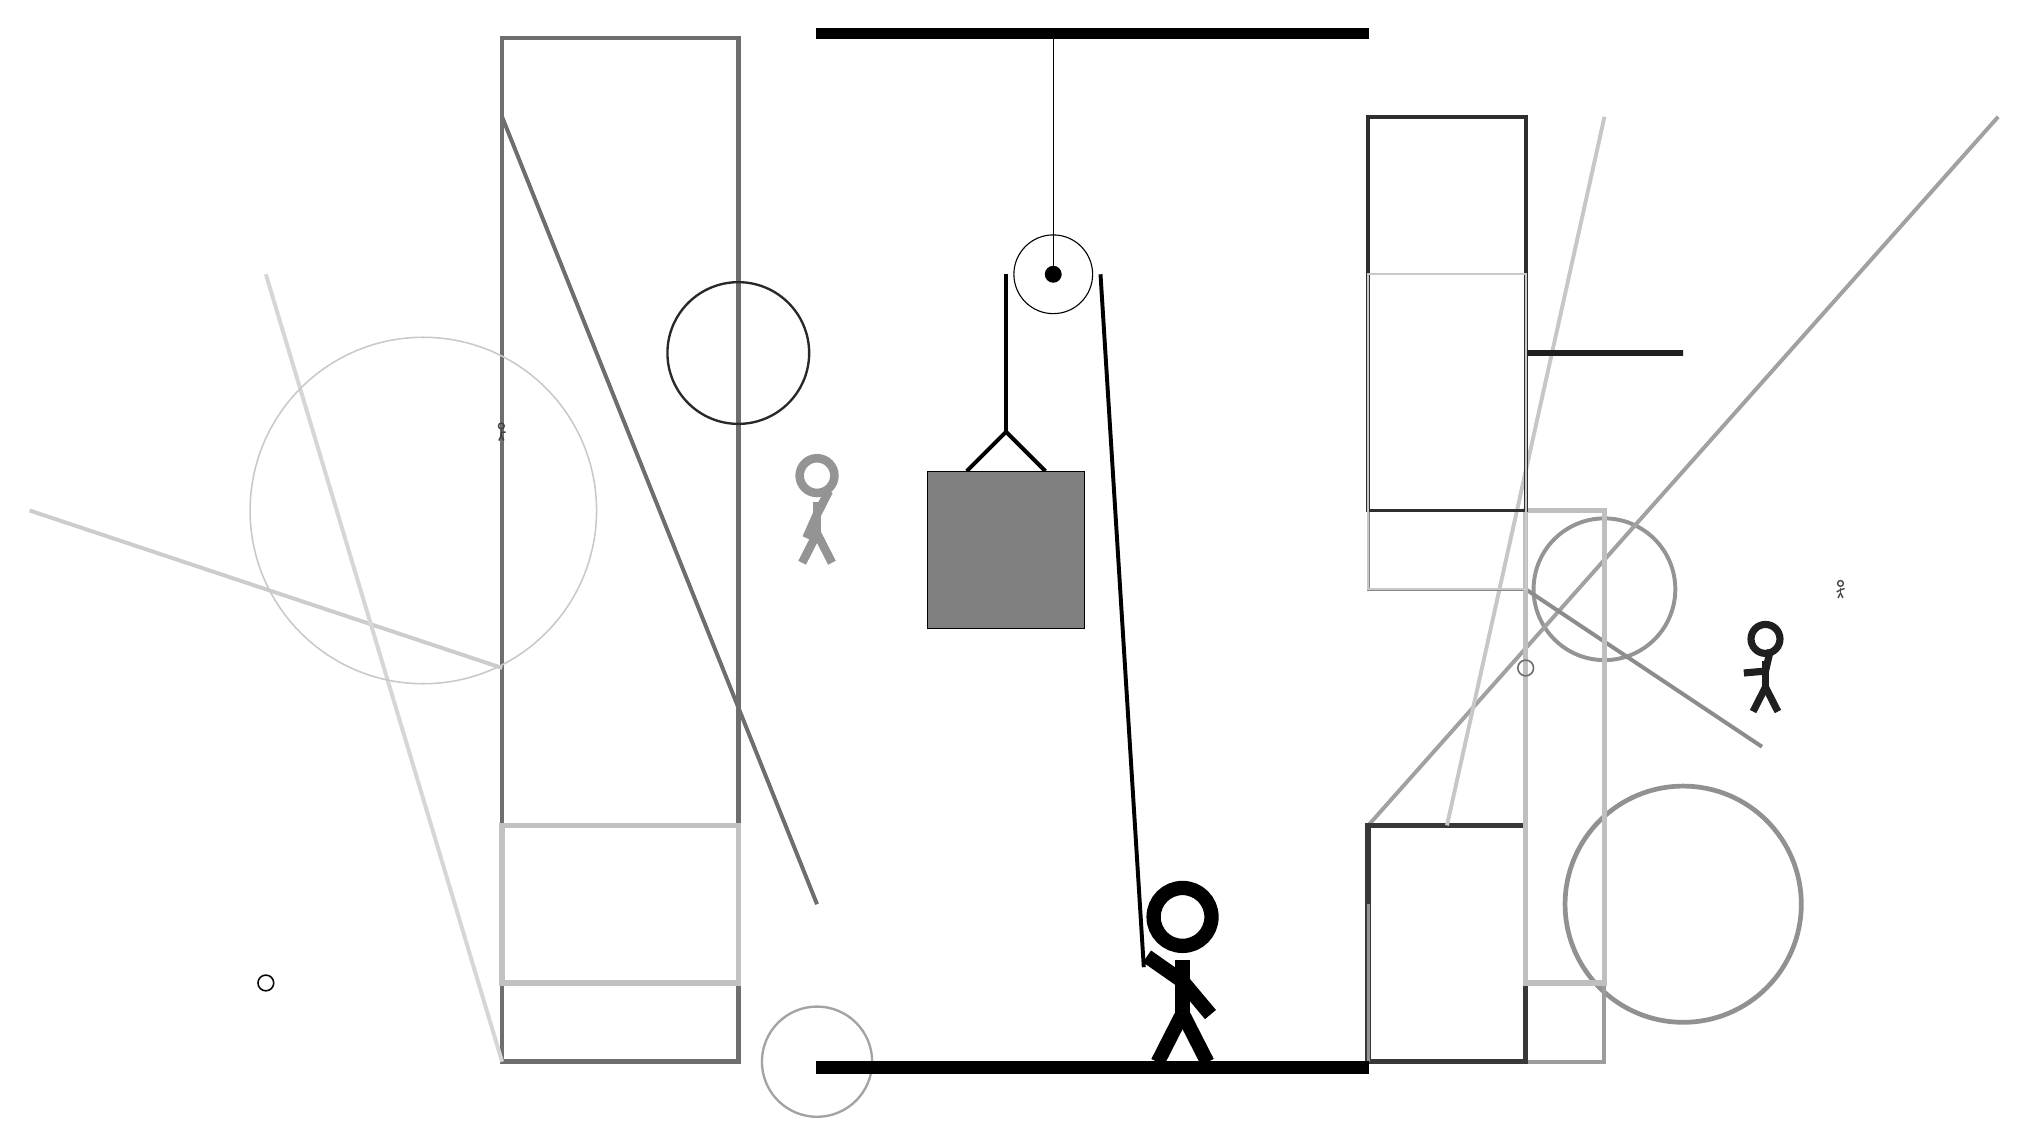
\begin{tikzpicture}
		%%%%% START %%%%%
		
		\draw[fill=black] (-2, 10) rectangle (5, 10.125);
		
		\draw (1, 7) circle (0.5);
		\draw[fill=black] (1, 7) circle (0.1);
		\draw (1, 10) -- (1, 7);
		
		\draw [line width=0.6mm, color=black!43](9, -1) circle (1.5);
		
		\draw[line width=0.6mm, color=black!57] (-3, 10) rectangle (-6, -3);
		\draw[line width=0.4mm, color=black!54] (5, 0) rectangle (5, -1);
		\node[line width=0.4mm, color=black!71] at (11, 3) {\Strichmaxerl[1][28][18]};
		
		\draw[line width=0.7mm, color=black!25] (6, 3) rectangle (6, 3);
		\draw[line width=0.5mm, color=black!39] (7, -3) rectangle (8, -2);
		\node[line width=0.4mm, color=black!75] at (-6, 5) {\Strichmaxerl[1][81][5]};
		\draw [line width=0.3mm, color=black!84](-3, 6) circle (0.9);
		\node[line width=0.6mm, color=black!42] at (-2, 4) {\Strichmaxerl[6][66][63]};
		\draw [line width=0.5mm, color=black!42](8, 3) circle (0.9);
		\draw[line width=0.5mm, color=black!20](-6, 2) -- (-12, 4);
		
		\draw[line width=0.5mm, color=black!37](5, 0) -- (13, 9);
		\draw [line width=0.3mm, color=black!36](-2, -3) circle (0.7);
		
		\draw[line width=0.7mm, color=black!78] (5, -3) rectangle (7, 0);
		\draw[line width=0.5mm, color=black!16](-6, -3) -- (-9, 7);
		\draw[line width=0.5mm, color=black!22](6, 0) -- (8, 9);
		
		\node[line width=0.6mm, color=black!88] at (10, 2) {\Strichmaxerl[5][5][77]};
		\draw[line width=0.5mm, color=black!45](7, 3) -- (10, 1);
		\draw[line width=0.4mm, color=black!47] (5, 3) rectangle (7, 9);
		\draw[line width=0.7mm, color=black!25] (7, 4) rectangle (8, -2);
		\draw[line width=0.5mm, color=black!82] (5, 4) rectangle (7, 9);
		
		\draw [line width=0.2mm, color=black!58](7, 2) circle (0.1);
		
		\draw [line width=0.2mm, color=black!98](-9, -2) circle (0.1);
		\draw[line width=0.5mm, color=black!57](-6, 9) -- (-2, -1);
		\draw[line width=0.7mm, color=black!88] (7, 6) rectangle (9, 6);
		
		\draw [line width=0.2mm, color=black!21](-7, 4) circle (2.2);
		\draw[line width=0.4mm, color=black!42] (5, -3) rectangle (5, -1);
		\draw[line width=0.7mm, color=black!24] (-3, -2) rectangle (-6, 0);
		\draw[line width=0.3mm, color=black!21] (5, 3) rectangle (7, 7);
		
		
		\draw[line width=0.5mm] (-0.1, 4.5) -- (0.4, 5.0) -- (0.9, 4.5);
		\draw[fill=black!50] (-0.6, 4.5) rectangle (1.4, 2.5);
		
		\draw[line width=0.5mm] (0.4, 7) -- (0.4, 5.0);
		\centerarc[line width=0.5mm](1, 7)(0:180:0.6);
		\draw[line width=0.5mm](1.6, 7) -- (2.15, -1.8);
		
		\node at (2.6, -1.9) {\Strichmaxerl[10][-35][-50]};
		
		\draw[fill=black] (-2, -3) rectangle (5, -3.15);
		
		%%%%% END %%%%%
	\end{tikzpicture}
\end{document}